\documentclass{scrartcl}

%\usepackage[utf8]{inputenc} % use UTF-8 as input encoding - not necessary with xelatex
\usepackage[T1]{fontenc} % make non-ASCII characters cut&pastable in PDF
\usepackage{lmodern} % easiest way to get outline fonts with T1 encoding
\usepackage[english=american]{csquotes} % automatic quotation style
\usepackage[american]{babel}

\usepackage{amsmath,amssymb} % math
\usepackage{caption} % For caption*
\usepackage[hidelinks, colorlinks=true]{hyperref} % Make links from things

\usepackage{graphicx} % images
\DeclareGraphicsExtensions{.eps,.pdf,.png,.jpg,.gif}
\graphicspath{{./img/}}
\usepackage{tabularx} % tabulars
\usepackage{array,booktabs} % rules for frontpage
\usepackage{titling} % "vars" for titlepage

% Setup the page geometry
\usepackage[a4paper,top=3cm,bottom=3cm,left=3cm,right=3cm]{geometry}
%\usepackage[a4paper,margin=5cm,top=3cm,bottom=3cm,left=2.7cm,right=2.7cm]{geometry}



\title{AURsec}
\newcommand{\titlesub}{A blockchain aproach to securing software packages }
\author{Bennett Piater \& Lukas Krismer}
\newcommand{\leader}{Supervisor: Christian Sillaber}
\newcommand{\university}{University of Innsbruck}
\newcommand{\course}{Bachelor thesis}
\date{\today}

\begin{document}
  %%% Boilerplate
  \thispagestyle{empty}

  %frontpage
  \begin{titlepage} 
    \noindent
    \begin{tabular}{@{}p{\textwidth}@{}}
        \toprule[2pt]
        \midrule
        \vspace{0.15cm}
        \begin{center}
            \Huge{\textbf{\thetitle}} \\
            \normalsize{\titlesub} 
        \end{center}
        \vspace{0.15cm}\\
        \midrule
        \toprule[2pt]
    \end{tabular}
    \vspace{4 cm}
    \begin{center}
        \vspace{0.2cm}
        \LARGE{\theauthor} \\
        \vspace{0.1cm}
        %{\small \matrikel}
    \end{center}
    \vfill
    \begin{center}
        \course \\
        %\group \\
        \leader \\
        \vspace{1.2 cm}
        \university
    \end{center}
\end{titlepage}


  % TODO: Do we really need that ?? we have the frontpage
  \vspace*{\fill}
  \begin{center} \textbf{\large{STATUTORY DECLARATION}} \end{center}
  I declare that I have authored this thesis independently, that I have not used other than the declared sources  /  resources,  and  that  I  have  explicitly  marked  all  material  which  has  been  quoted  either literally or by content from the used sources.

  \begin{center}
  \begin{table}[!htb]
  \begin{tabularx}{\textwidth}{lXX}
  Innsbruck 17.05.2017 & \_\_\_\_\_\_\_\_\_\_\_\_\_\_\_\_\_\_ & \_\_\_\_\_\_\_\_\_\_\_\_\_\_\_\_\_\_ \\
  Location,Date & Bennett Piater & Lukas Krismer \\

  \end{tabularx}
  \end{table}
  \end{center}
  \vspace*{\fill}
  \pagebreak


  \pagenumbering{Roman}
  \begin{abstract}
  % TODO
  \end{abstract}

  \tableofcontents
  \listoffigures
  \listoftables
  \pagebreak


  %%% Content starts here
  \pagenumbering{arabic}

  \section{Introduction}  %(1/2 page)
  The Linux distribution Arch makes it easy to create custom packages and has a very active community. Because of this, there was the need for a place where users could upload their packages for others to use.

  ftp://ftp.archlinux.org/income was created, where packages could be put until maintainers that were willing to do so could adopt them, but this delay was too long, so another solution was needed.
  The next improvement were the Trusted User Repositories, where some privileged users, which were many more than the maintainers of before, were allowed to host their own repositories for anyone to use.

  The \emph{Arch User Repository} were the natural evolution: By removing all middlemen, everyone can now upload their packages to one central place. \cite{wiki:AUR}

  The AUR is similar to PyPI (Python), NPM (Javascript) and rubygems.org, where all users can share their packages. They all share the problem that submitted packages are not necessarily audited or even checked by anyone.

  \section{Security Issues of the AUR} %(1 1/2 pages)
  Indeed, ease of use appears to have been, if not the only, at least the primary design consideration of the Arch User Repository. This creates so many security issues that it is actually quite a task to think through all of them.

% PKGBUILDS
\subsection*{Local Package Creation}
One of the most obvious problems is the installation procedure itself.
The AUR doesn't host binary packages, which is a good thing. Instead, Arch packages are created locally from a bash file, the so-called \texttt{PKGBUILD}, containing metadata like name and version, the URLs and checksums of upstream sources, and functions for the compilation and packaging steps. % TODO: We may want to show an example PKGBUILD somewhere - but where? Maybe as appendix, with reference from here?

The AUR contains these \texttt{PKGBUILDS} and possible patches to be applied to the upstream sources in a git repository per package.
A package file can be produced by cloning it's repository and using a tool called \texttt{makepkg} \cite{wiki:PackageCreation}, which sources the script, downloads and verifies the sources, and calls the compilation and packaging functions.

This means that users can verify what they are compiling as opposed to blindly trusting binaries created by third-parties, but also that maintainers of AUR packages have a means of executing arbitrary shell commands on users' machines.

This is aggravated by the fact that \texttt{PKGBUILDS} can include a \texttt{.install} file into the built package, which will be executed \emph{as root} when the package is actually installed.
The risk also increases if so-called \enquote{AUR helpers} are used. These tools assist the users in installing packages from the AUR by automating the steps and behave like package managers.
Some of them (notably \texttt{aurutils} \cite{gh:aurutils}, which is recommended by the authors) allow the users to inspect these files before continuing, but others are very unsafe in that they execute code before giving users the opportunity to inspect it, or decentivize them from doing so.

\subsection*{The Trust Issue}
Another problem is that users are not given any reason to trust the maintainers.
Unlike the official repositories, where maintainers are vetted, packages are (often manually) audited before being accepted, and everything must be signed with a trusted OpenPGP key, anyone can create an account and submit a new package to the AUR in a few minutes.
There is no admission procedure or audit system and no OpenPGP web of trust in order to minimize the time needed to publish a package or update.

\texttt{makepkg} can verify OpenPGP signatures for upstream sources, but the \texttt{PKGBUILD} itself could only be signed by using signed git commits, which is sadly not enforced or even officially recommended --- and not supported by any AUR helper anyway.

Except when using the AUR helper \texttt{bauerbill} \cite{bauerbill}, which provides a basic user-side trust management system, the only way to be maintain reasonable trust is therefore to manually read every single file, which is cumbersome.
Because only highly security-conscious users are willing to put in so much effort before trusting a \texttt{PKGBUILD}, most users are left vulnerable by the aforementioned issues.

\subsection*{Adopting orphan packages}
The trust issue is made even worse by the fact that packages can silently and quickly be taken over by other maintainers due to the orphan/adoption system.

When a maintainer wants to stop maintain a package, but the package is still useful and actively developed upstream, he has the option to \emph{orphan} it rather than deleting it.
Orphan packages can be \emph{adopted} by any AUR user, at any time, without delay.
This feature was designed to minimize update delay, which it does effectively; However, it also makes it easy for malicious agents to take over popular orphaned packages, manipulate them, and immediately orphan them afterwards.

\begin{figure}
	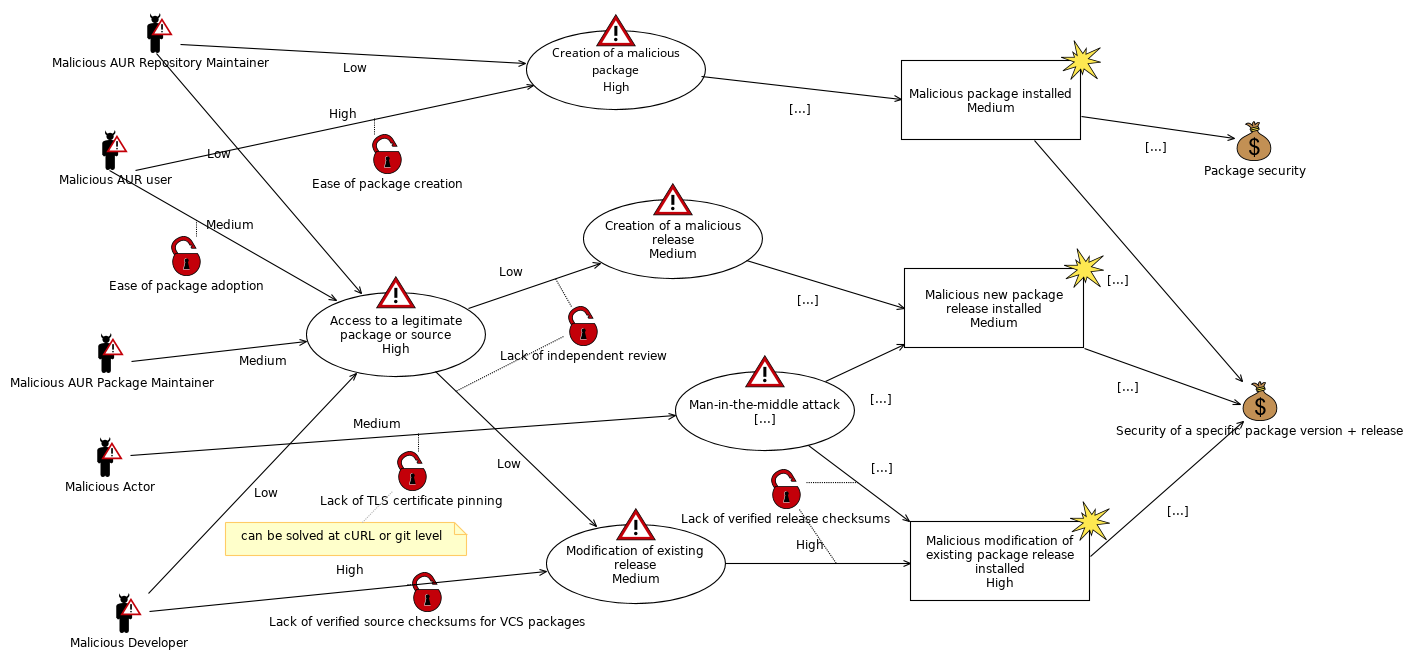
\includegraphics[width=\paperwidth]{img/threat.png}
	\caption[Threat Assessment]{Threat Assessment of the Arch User Repository}
	\label{fig:threat}
\end{figure}

\subsection*{Concrete Attack Scenarios}
We used the CORAS \cite{Dahl:2007} threat modeling language to arrange the security issues in such a way that concrete attack scenarios are intuitive to comprehend and retrace. The resulting threat diagram can be seen in Figure~\ref{fig:threat}.

Many of the AUR's security issues exist by design and are only included for completeness. However, several issues lead to the same situations; This means that security issues further along the right of the diagram tend to be more promising candidates in the search for solvable problems.

This knowledge leads to two concrete attack scenarios that could be preempted without redesigning the AUR, which are outlined below.

% Threats:
\subsection*{Tampered VCS Sources: Malicious Upstream}
In some cases, the user is not adequately protected against malicious (or compromised) upstreams:

The AUR supports so-called \emph{VCS packages} \cite{wiki:VCSPackages}, which download sources from a version control system, such as Git or Mercurial, instead of downloading a fixed archive. This relieves the maintainer from updating his \texttt{PKGBUILD} for every new commit.
\texttt{makepkg} will even automatically calculate the up-to-date version number using e.g. tags and commit numbers.

VCS packages were primarily designed to simplify the installation of up-to-date packages from source, and they do that very well; But they also introduce a big security issue:
Since the \texttt{PKGBUILD} must not be updated between versions, it cannot contain checksums for the new version, either.
This means that users don't have a way to verify the authenticity of the source that they are downloading, unless they can trust the upstream himself, meaning that no-one will notice if the upstream is compromised or makes malicious changes. There is no way to defend against this except to manually audit the upstream sources, which should primarily be the maintainers responsibility.

\subsection*{Tampered Packages: Malicious Maintainer}
Users are also not adequately protected against malicious maintainers:

Because it's so easy to gain access to a package, e.g. by adopting an orphan or simply by creating it, and nothing is verified or audited before publication, It's easy for a malicious agent to modify a package.
And because the \texttt{PKGBUILD} is not signed or hashed, users will not notice if the build instructions for a specific package version were modified. This allows targeted attacks:

If the time at which a target will update his machine is known and one has access to an AUR package which he is expected to update, malicious code can somehow be introduced into the corresponding \texttt{PKGBUILD} within that update window.
This could be as simple as changing the checksum if one also has access to the upstream source code (even a very careful user has no chance of noticing this attack), or executing innocuous code in the install file or \texttt{PKGBUILD} itself.

The malicious change could be reverted immediately afterwards. If the time frame is short, no other AUR user (and thus, \emph{no-one}) would ever notice.
One could only defend against this with a good local trust model, such as that possible with \texttt{bauerbill}, or manual cryptographic verification of the git commit to the AUR --- assuming that the maintainer signs his commits, which is only very rarely the case.
 % BENNETT

  \section{The Solution} %(4 1/2 pages)
    \begin{figure}
      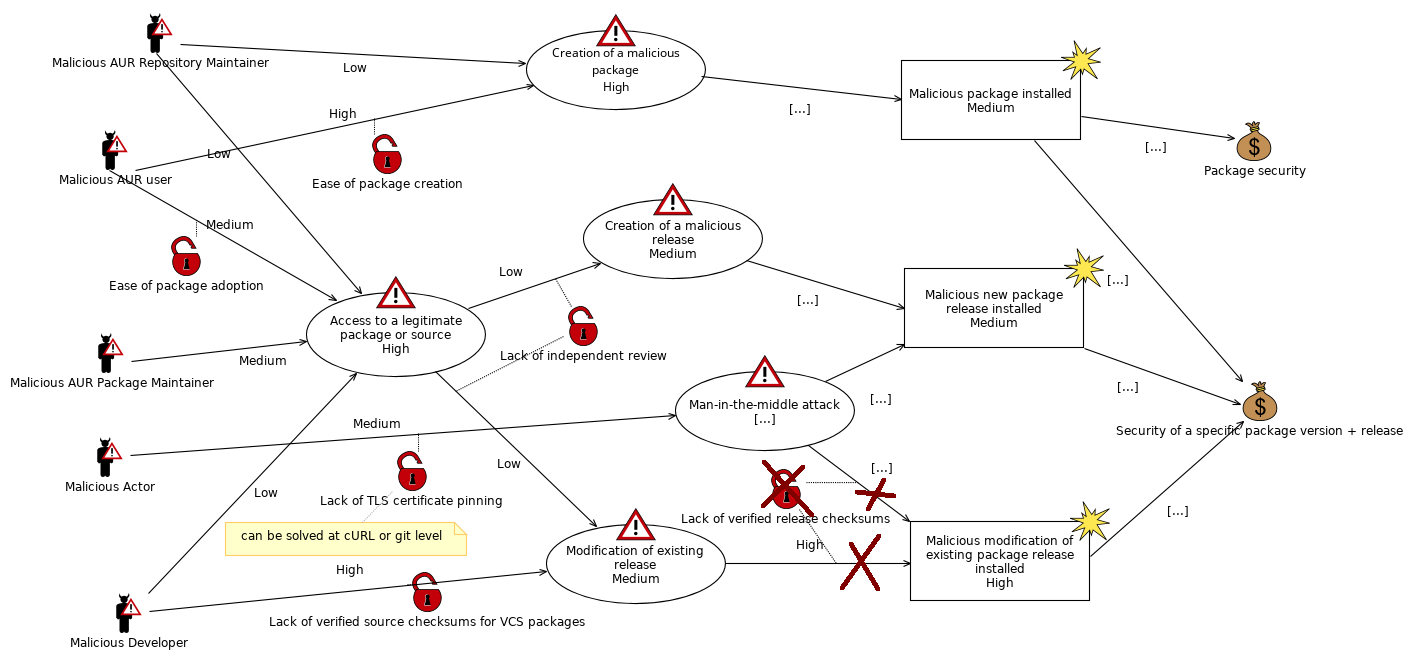
\includegraphics[width=\paperwidth]{img/threat2.png}
      \caption[Threat Prevention Strategy]{Strategy for Improving the Security of the AUR}
      \label{fig:threat2}
    \end{figure}

    Defence against the two attacks mentioned above requires the availability of cryptographically secure release hashes for every version of every package; If those were available, an attack would result in a hash mismatch and therefore warn the user. However, the AURs design prevents any secure implementation on the server side.

    \subsection{Core Solution}  %(1 page)
     % Die Lösung einiger Security-Probleme, ist eine sichere Datenbank, die die Hashs der versionierten Packete beinhaltet. Bevor man ein Packet installiert können der lokal generierte Hash mit jenem aus der Datenbank verglichen werden, um sicherzustellen, das das Packet das selbe wie bei anderen Usern ist. 

 % Um die Datenbank so sicher wie möglich zu gestalten, wird eine Blockchain eingesetzt auf der ein Smart Contract liegt. Dieser smart Contract ermöglicht die Verwendung von Funktionen auf der Blockchain. Mit diesen Funktionen können neue Hashes in die Blockchain geladen werden und es kann der derzeitige Hash eines Paketes und dessen Anzahl abgefragt werden. Hierbei wird garantiert, das von jedem Nutzer für eine Paketversion immer nur ein Hash existiert. Dies ist die erste bekannte Verwendung einer Blockchain für ein solches Problem.

% Der Workflow

% Bild 1 einfügen 
% Bild 2 einfügen

% 1) Zuerst wird ein PKGBUILD heruntergeladen und in einer Sandbox teilweise ausgeführt. Die so erhaltenen Daten werden anschließend gehashed. 
% 2) Dann wird der Hash mit dem (current consens) Hash des Paketes aus der Blockchain Verglichen (siehe Bild 2). Wenn diese überein stimmen und die Anzahl der commits über dem Threshold liegt wird \texttt{true} zurückgegeben. Ansonsten kann man selbst entscheiden ob man dem lokal generierten Hash vertrauen will oder nicht. 
% 3a) Wenn dem Hash vertraut wird kann man sein Paket installieren. Bei dieser Option wird dann der Hash mit der versionierten Packet ID an die Blockchain gesendet und in dieser aufgenommen, insofern dieser User für diese PacketID noch keinen Hash commited hat.
% 3b) Wenn dem Hash nicht komplett vertraut wird, kann man trotzdem das Packet installieren, schickt aber den Hash nicht an die Blockchain.
% 3c) Wenn dem Hash nicht vertraut wird, baut man das Packet anschließend nicht.
% 4) Diese Transaction wird dann an alle Nodes der Blockchain geschickt.
% 5) Sobald eine der Nodes einen neuen Block mined, wird die Transaktion validiert und in der Blockchain verinnerlicht.

% Intro
The solution for a few security-problems is a secure database, which contains hashes of versionized packages. Before a package is installed, the locale generated hash can be compared with the one in the database. This guarantee that the loaded package is the same as the package loaded by most of the other users.

To make the database as safe as possible, a blockchain is used. On this blockchain is a smart contract, which allows to call functions. With one of these functions it's possible to commit hashes of versionized packages. This hash will be saved in the blockchain if this user has not committed a other hash for the same versionized package before. Another function is used to get the current consensus hash and its number of commits of a versionized package. This is the first application which uses a blockchain to secure downloads.

% Workflow
\subsection*{Workflow}
The following workflow is visualized by Figure \ref{fig:main_workflow}.
\begin{figure}
	\centering
		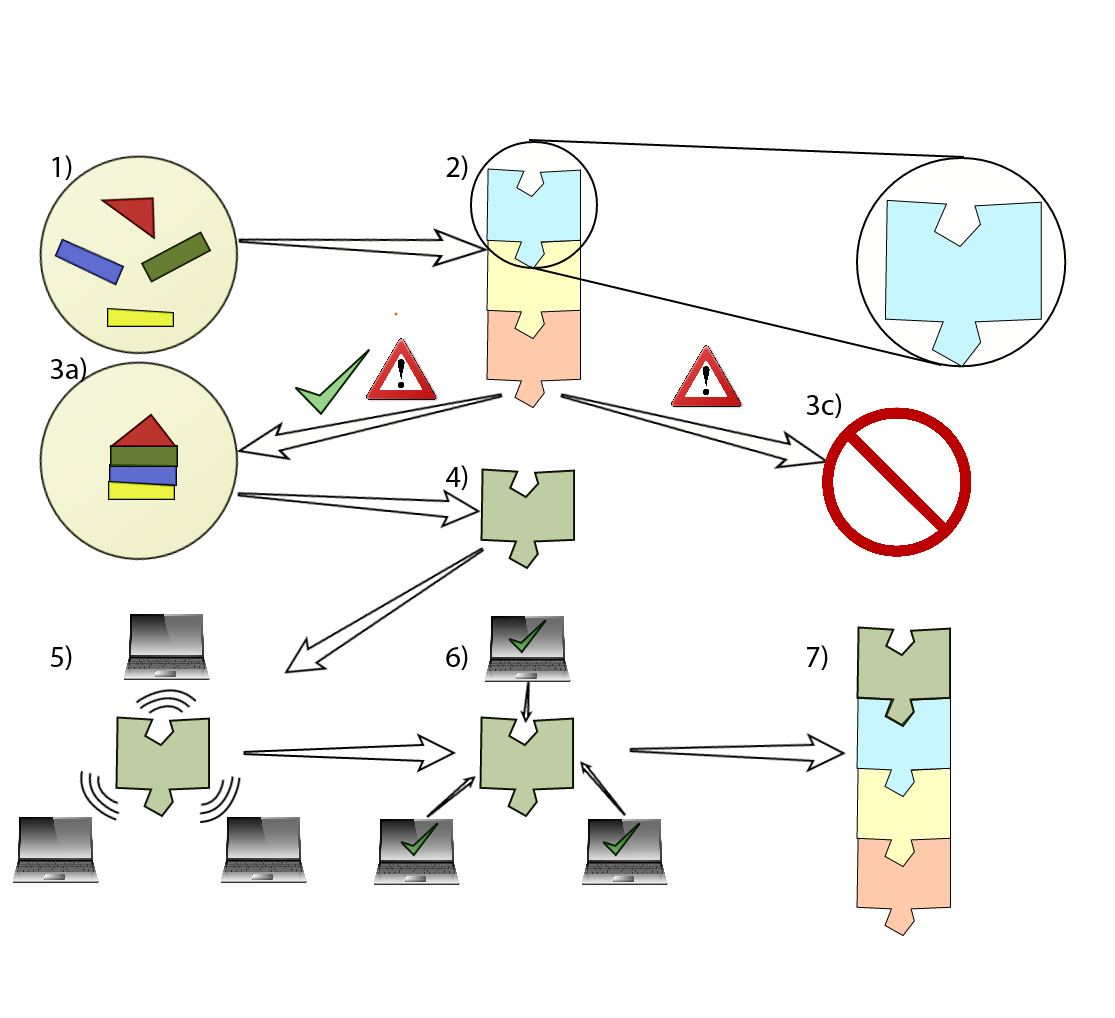
\includegraphics[width=0.6\paperwidth]{Workflow2}
	\caption{Main Workflow}
	\label{fig:main_workflow}
\end{figure}

\begin{figure}
	\centering
		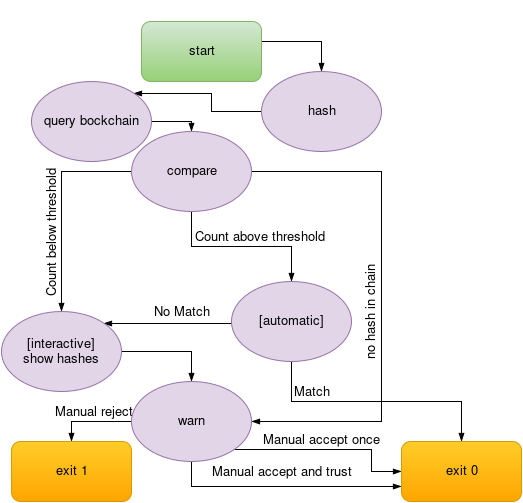
\includegraphics[width=0.45\paperwidth]{workflow}
	\caption{Decision Workflow}
	\label{fig:decision_workflow}
\end{figure}


\begin{enumerate}
	\item First of all a \textit{PKGBUILD} is downloaded and partially executed in a virtual area. Then this data get hashed. 
	\item The resulting local hash becomes compared with the current consensus hash of the versionized package of the blockchain [Figure \ref{fig:decision_workflow}]. 
	\item Now the workflow splits into 3 different paths.
	\begin{itemize}
		\item a) The hashes match and the number of commits is over the threshold or the user decides to trust the local generated test. The package is created and installed. \textit{(Followed by step 4.)}
		\item b) The hashes don't match and/or the number is below the threshold but the user want to create and install the package. \textit{(End of the workflow.)}
		\item c) The hashes don't match and/or the number is below the threshold and the user doesn't want to create the package. \textit{(End of the workflow.)}
	\end{itemize}
	\item The local hash is committed to the blockchain (this is a transaction).
	\item All nodes of the blockchain-network get the transaction.
	\item The transaction is contained in the next mined block.
	\item The block is added to the blockchain.
\end{enumerate} %LUKAS
    \subsection{Detailed Description} %(2 pages)
    \subsubsection{Blockchain} \label{sec:blockchain}

\subsubsection*{general}
The following paragraphs are based on \emph{Blockchain Beyond Bitcoin} \cite{Underwood}.

A blockchain is a distributed database system which is not owned by a single user. Every user can see all transactions. If a user wants to add a transaction to the blockchain, the transaction is encrypted and sent to all users. The transaction is then verified. If the majority of the users validate the transaction, the data is added to the blockchain in a block. ``Transactions are secure, trusted, auditable, and immutable''. Blockchains do not need backups because every user has his own copy which is synchronized with all other blockchains in the network.

\paragraph*{Smart Contracts} are using computerized transaction protocols to execute the terms of the contract which are agreed by the users. They are executed by every miner. Since their code is in the chain, it is guaranteed to be immutable and therefore impossible to manipulate. This means that one is effectively able to run code on the blockchain.

\subsubsection*{specific}
Our blockchain has to fulfill several requirements:
\begin{itemize}
	\item Since we target Arch Linux, it should be easy to install on this platform.
	\item It needs to provide an API which allows external scripts to work with it.
	\item It needs to provide smart contracts to maintain the constraints of the hash storage.
	\item It needs to provide an easy way to create private networks seperate from the main one, because full networks are huge.
\end{itemize}

The blockchain of choice was Ethereum because it is the only production-ready infrastracture providing smart contracts. It even allows them to be written in a high-level language, \emph{Solidity}, which makes them straightforward to write and understand.

\paragraph*{smart contracts}
Aursec has two smart contracts. The first one is a formal contract, which allows the owner of the contract to delete the contract. The second contract is a child of the first. In this contract are the ``user-functions'', which allows all users to send hash-commits and request the current consensus hash of a versioned package. The Contract allows a user to commit one hash per versioned package. Further commits of hashes of the same versioned package will not be considered. The current consensus of a versioned package is the most often committed hash so the hash of a package is not fixed by the first commit.

\paragraph*{network}
Like other blockchains, the Ethereum network is peer-2-peer, but private networks need to provide their own \emph{bootnode} through which peers announce themselves. Our bootnode is active 24/7 on a DigitalOcean droplet provided by our supervisor.

\paragraph*{interfaces}
The Ethereum blockchain provides 2 different interfaces, the IPC (interprocess communication), which provides an interactive javascript shell, and the HTTP RPC (remote procedure call) interface. The IPC interface of our blockchain is deactivated because users do not need to manually use the javascript shell: the only required interaction with the blockchain is through the shell script \texttt{aursec-chain}~(Section~\ref{sec:aursec-chain}) and the Python script \texttt{aursec-tui}~(Section~\ref{sec:tui}). These scripts communicate with the blockchain trough the RPC interface.
 %LUKAS
    \subsubsection{aursec-init}
Aursec-init is a shellscript which allows the user to create all requirements just by running it. It also allows to overwrite an existing aursec-blockchain with a new one.

% TODO add refs
\paragraph*{workflow of the initialization:}
\begin{enumerate}
	\item Create needed folders and markers (markers are needed by TODO)
	\item Create the blockchain from our genesis block.
	\item Create a new user with a random password which is saved in a file.
	\item Create the \emph{Directed Acyclic Graph} for the blockchain, which is a ~1GB dataset. The DAG is needed for mining new blocks. \cite{wiki:DAG}
	\item Set safe permissions for the above files and folders.
	\item Mine a few blocks to trigger the synchronization and to have enough ether to be able to commit a few hashes from the start. % TODO: @lukas If you use the word ether here, you need to explain it!
\end{enumerate}
 %LUKAS
    % aursec systemd services  ||| BENNETT
    \subsubsection{aursec --- Architecture}
We designed \texttt{aursec} to be a good UNIX citizen:

\begin{itemize}
\item Modular design \\ multiple small tools doing one thing and doing it well
\item Adherence to the universal interface \cite{Salus:1994} \\
  Work on streams of text on \texttt{stdin} and \texttt{stdout}
\item Written in Bash and using existing tools where possible
\item Maximize concurrency using a pipeline
\end{itemize}

\texttt{aursec} builds a pipeline of two other tools, \texttt{aursec-hash} and \texttt{aursec-verify-hashes}, which produces lines containing the id and hash of a package as well as the hash representing the current consensus on the blockchain and the number of times that hash was submitted.
It then inserts itself into that pipeline and iterates over the lines of items using a \emph{while-read} loop and traverses the aforementioned state machine for each item.

This architecture has several advantages: It is straightforward to understand because it follows standard UNIX patterns, which also makes it very maintainable.
The free 3-level parallelism gained by the pipeline is a very useful advantage in itself, but even more so because all 3 tools are primarily I/O-bound: \texttt{aursec-hash} reads and hashes lots of files, \texttt{aursec-verify-hashes} constantly queries (and waits for) the blockchain, and \texttt{aursec} tends to spend much time waiting for user input.
Thus, the concurrency is even more important because it allows work to continue in the background while \texttt{aursec} waits for the user. Indeed, the background tasks tend to be finished in most practical situations before the user has had time to inspect the second or third warning. % NOTE: Maybe add an anecdote about how this is similarly good to the bulk-verification of sources in aursync vs yaourt?

\subsubsection{aursec-hash}
\texttt{aursec-hash} has the simple task of producing an ID (\texttt{$pkgname-$pkgver-$pkgrel}) and a hash from \texttt{PKGBUILD}s.

The id could be parsed from the \texttt{.SRCINFO}, which is a plain text file.
But VCS packages don't have up-to-date version information in their \texttt{PKGBUILD}, which means that it must be interpreted; This is annoying, but we only source the \texttt{PKGBUILD} in a \texttt{firejail} sandbox to minimize the inherent risk of executing foreign turing-complete code.
This allows us to get an accurate ID for VCS packages, but also to include the actual sources in the hash, thereby compensating for the lack of hashes in the \texttt{PKGBUILD} of VCS packages.

The \texttt{PKGBUILD} is hashed after stripping it's comments, and VCS sources, if they exist, are hashed using \texttt{find}.
Finally, all hashes are combined by another call to the hash command.
Currently, \texttt{sha256sum} is used for it's good speed and security.

\subsubsection{aursec-verify-hashes}
This tool is not very interesting; It simply fetches the current consensus for every package ID on \texttt{stdin}, computes whether it matches with the locally computed hash, and appends that data to the output stream.
Doing this in a separate pipeline step is very worth it because requests from the blockchain are comparatively slow.

    % aursec{,-hash,-verify-hashes}   ||| BENNETT
     \subsubsection{aursec-chain}\label{sec:aursec-chain}
Aursec-chain is a shellscript which allows the user to intergate with the blockchain. The script itself communicate with the blockchain through JSON RPC. To provide the user all needed commands, the script has different arguments.

\paragraph*{mine}
This argument needs more arguments to work.
\begin{itemize}
	\item \texttt{start:} Starts mining.
	\item \texttt{stop:} Stops mining.
	\item \texttt{N blocks:} wait till mining is stopped and then mines N blocks.
	\item \texttt{auto:} this argument is just used by a systemd service to mine blocks periodical.
\end{itemize}

\paragraph*{commit-hash}
This argument needs two more arguments to work. The first one has to be the versionized package id and the second has to be the local generated hash of the package. The script then sends a transaction to the blockchain (if enough ether is available). This transaction will be verified by the next mined block.

\paragraph*{get-hash}
This argument needs one more argument to work. This argument has to be the versionized package id. Then aursec-chain calls a method which returns the current consensus hash and the number of commits of this hash. 
 %LUKAS
    % TODO: what else
    \subsection{Terminal User Interface} %(1/2 page)
    \label{sec:tui} % TODO: Mention which TUI library you used!
\texttt{aursec-tui} is a Python script. The TUI gives an overview over all mined blocks, their hashes, the miner of the block and eventual transactions which are saved in the block.

It is split in two parts. The first part is needed to gain the data from the blockchain and save it, the other part formats the information and displays it. To display the results as fast as possible a thread searches the blockchain in the background. Any additional data will be displayed after the next refresh. The script offers the user two settings for filtering the results.
\begin{itemize}
	% TODO: während ich das lese fällt mir auf, dass du die Optionen umbenennen solltest :)
	\item \texttt{only mine:} only display blocks which where mined by the user himself.
	\item \texttt{only transactions:} only display blocks with transactions.
\end{itemize}
The settings can be combined with the result that all blocks mined by the user with transactions will be displayed.

    \subsection{Project Management} %(1 page)
    % TODO: @lukas this paragraph seems kind of useless, can we think of something better to say?

This project was done by three people: Two students who implemented the tool and their superior. So there had to be a lot of communication. The communication tools were offline meetings, Slack and emails. For filesharing Github is used.

%\paragraph*{Slack} is an web-based instant-messaging-service especially for team-projects. For this Project a channel with two integrations was used. The first integration is the Github integration, with shows all activities on a github repository. The other one is the circlecl integration, which shows the result of the CI-tests.

\subsubsection*{timeline}
From the timeline (Figure \ref{fig:timeline}) can be derived that this project was realized in less then 9 months. The real worktime exposure ratio of the three main-task (reading, programming and writing) differs extremely from the visualized one. In reality we read 50\%, programmed 40\% and wrote 10\% of the worktime.
It is also visible that we didn't manage to complete three milestones in time. This was caused by different circumstances, but we managed to complete the hole project in time cause we adjusted our planing every few weeks.

\begin{figure}[!htb]
	\centering
		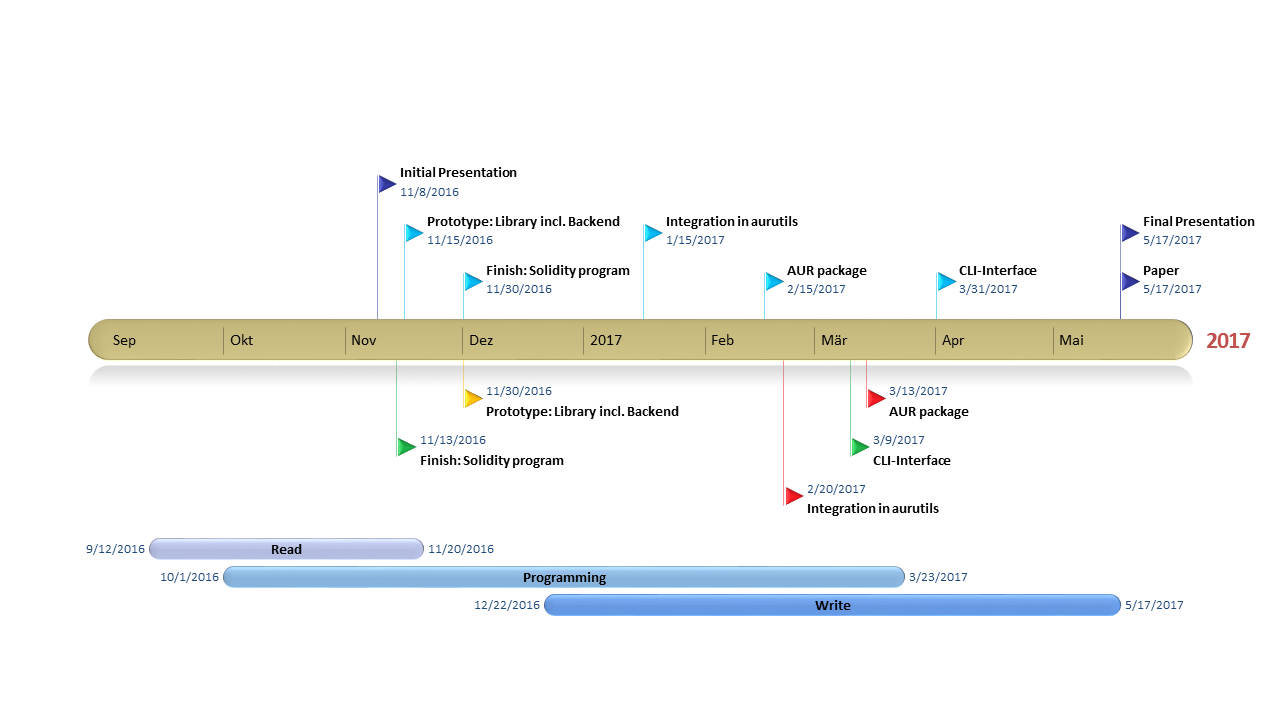
\includegraphics[width=0.7\paperwidth]{timeline}
	\caption{Timeline}
	\label{fig:timeline}
\end{figure}


% Notes:
% TODO: Add refs
 % LUKAS
    % TODO: What else?

  \section{Things we Learned} %(1 page)
  % Ethereum - Solidity
% RPC
% Bash as a programming language
% Python - Urwid

\subsubsection*{Ethereum --- Solidity}
Programming on a blockchain is a very interesting concept, but it also takes some getting used to. Thankfully, Solidity is a cleanly designed language which abstracts the blockchain away very nicely.

In practice, writing for Ethereum turned out to be enjoyable. Solidity reads like a half-way mix between C and Javascript, and most things that we rely on in this project happen automatically: Guaranteeing that the code cannot be modified, the ACID properties of transactions, etc.
This means that Ethereum, and Solidity in particular, are ideally suited for secure, \enquote{intelligent} (self-enforcing) databases.

Because of that, our code reads largely like a pseudo-code description of the algorithm itself, making it easier to maintain and verify.
Solidity even supports some automatic formal verification, but not yet for \texttt{struct}s, so we cannot make use of it for our program.

\subsubsection*{JSON RPC} % TODO: @lukas I'm not sure whether this is interesting enough to be mentioned here?
The JSON PRC is used by the aursec-ethereum-blockchain for remote access to the block. Methods can be called or transactions can be sent by sending a JSON-Object to the block chain. The answer from the block chain is also always a JSON-Object. One big advantage is the easy parsing from and to JSON-Objects both in Bash and Python. The best example is visible in the code of aursec-tui (Section~\ref{sec:tui}).

\subsubsection*{Bash}
Using Bash as a programming language is interesting. The syntax can be weird, even arcane; At the same time, we were often surprised by the advanced features that are provided directly inside the language, such as string substitutions, regular expression matching or associative arrays.
In addition, the \texttt{coreutils} are very powerful; To our knowledge, only the Python standard library offers comparable functionality.

Apart from getting used to the uncommon syntax, we found that the most important prerequisite for writing larger programs in Bash was to think in streams:
Bash is not strictly imperative or functional, and it's certainly not object-oriented. Functions and programs can only return non-integer values as text on \texttt{stdout}, and it is often useful to provide them their input on \texttt{stdin} as well.
We quickly found out that the most efficient way to structure programs is to use \texttt{while-read} loops, which iterate over an input stream of text.

Embracing this design philosophy results in the natural use of highly concurrent pipelines that turn out to be very easy to understand, maintain and extend, far more so than equivalent imperative or object-oriented versions.
Readers familiar with Java can compare this to Java 8's \texttt{java.util.stream} API.

Writing safe and correct code is as hard as in C, mostly due to the lack of exception handling or a sensible alternative.
We work around that using \texttt{set -e}, which cancels a program whenever an unused return value is non-zero, and exit handlers for cleanup.

Bash doesn't provide or recommend a canonical testing framework, but associative arrays and \texttt{eval} allowed us to write our own system for basic unit tests with named test cases, commands to execute, and expected invariants.
We used it to great effect in narrowing down the best \texttt{firejail} sandbox ruleset, e.g. preventing \texttt{makepkg} from writing to folders other than \texttt{pwd}.

\subsubsection*{Python-Urwid}
Urwid is a \emph{Terminal User Interface} (TUI) library for Python. It provides ready-made widgets which make it easy to create structured user interfaces.

  % Ethereum - Solidity
  % RPC
  % Bash as a programming language
  % Python - Urwid
  % TODO: WHAT ELSE?

  \section{Evaluation} %(1 page)
  % We can probably already talk about our own experience? Our Data/ Data from outside ?

  %%% Content ends here
  \pagebreak
  % TODO: preferrably cite english pages
  \bibliographystyle{plain}
  \bibliography{Literature.bib}

\end{document}
